\chapter{Methods}

\section{Cetacean vocalization}

Many species of cetaceans can be found near Iceland.
There are at least 12 species of cetaceans that roam Iceland waters.
Among which are most frequently spotted are harbour porpoise, white beaked dolphins, minke whales and humpback whales \cite{user_whales_nodate}.
Sound is used by cetaceans for various purposes the low frequency sounds are used for communication and high frequency prey hunting, predator avoidance as well as echolocation for navigation \cite{nowacek_studying_2016}.
Each species can vocalize different sounds.
The sounds can be described as moans, calls, clicks, shrieks and more\cite{greenhow_hearing_nodate}.
%Cetaceans use these sounds to low frequency sound for communicating to one another all the way to creating high frequencies echolocation sounds for hunting their prey\cite{greenhow_hearing_nodate}.
Table \ref{Tab:WhaleHz} shows the type of sound, frequency range of the sound, the dominant frequency of the sound and the source level of each sound for its respective species.

\newpage


\begin{table}[]\caption{Frequency ranges of whales that are found near Iceland \cite{richardson_marine_2013}, * taken from \cite{richardson_effects_1991}}.\label{Tab:WhaleHz}
\centering
\resizebox{\textwidth}{!}{
\begin{tabular}{|l|l|l|l|l|}
\hline
\begin{tabular}[c]{@{}l@{}}Species \\ of \\ whale\end{tabular} & Noise type             & \begin{tabular}[c]{@{}l@{}}Frequency range\\ {[}Hz{]}\end{tabular} & \begin{tabular}[c]{@{}l@{}}Dominant \\ frequencies \\ {[}Hz{]}\end{tabular} & \begin{tabular}[c]{@{}l@{}}Source level \\ {[}dB re 1 $\mu$Pa at 1m{]}\end{tabular} \\ \hline
Blue    & Moans & 12 - 390 & 16 - 26 & 188 \\ \cline{2-5}
        & Clicks & \begin{tabular}[c]{@{}l@{}}  6k - 8k\\ 21k - 31k\end{tabular} & \begin{tabular}[c]{@{}l@{}}6k - 8k\\ 25k\end{tabular} & \begin{tabular}[c]{@{}l@{}}130\\ 159\end{tabular} \\ \hline
\begin{tabular}[c]{@{}l@{}}Bottlenose \\dolphin\end{tabular}    & Whistles & 0.8 - 24 & 4.5 - 14.5 & 125 - 173 \\ \cline{2-5}
        & \begin{tabular}[c]{@{}l@{}}Low-freq. \\narrowband\end{tabular}    & < 2 & 0.3 - 0.9 & - \\ \hline
Fin     & Moans, down sweeps & 14 - 118 & 20 & 160 - 186 \\ \cline{2-5}
        & Constant call & 20 - 40 & - & - \\ \cline{2-5}
        & Moans, tones, up sweeps & 30 - 750 & - & 155 - 165 \\ \cline{2-5}
        & Rumble & 10 - 30 & - & - \\ \cline{2-5}
        & Whistles, chirps & 1.5k - 5k & 1.5k - 2.5k & - \\ \cline{2-5}
        & Clicks & 16k - 28k & - & - \\ \hline
Harbour porpoises & Clicks & 2 & - & 100 \\ \cline{2-5}
        & Echolocation & 110k - 150k & - & 135 - 177 \\ \hline
Humpback & Song components & 30 - 8k & 120 - 4k & 144 - 174 \\ \cline{2-5}
        & Shrieks & - & 750 - 1.8k & 179 - 181 \\\cline{2-5}
        & Horn blasts & - & 410 - 420 & 181 - 185 \\ \cline{2-5}
        & Moans & 20 - 1.8k & 35 - 360 & 175 \\\cline{2-5}
        & Grunts & 50 - 1.9k+ & - & 190 \\\cline{2-5}
        & Pules trains & 25 - 1.25k & 25 - 80 & 179-181 \\ \cline{2-5}
        & Underwater blows & 100 - 2k & - & 158 \\\cline{2-5}
        & Fluke and flipper slap & 30 - 1.2k & - & 183-192 \\\cline{2-5}
        & Clicks & 2k - 8.2k & - & - \\ \hline
Minke & Down sweeps & 60 - 130 & - & 165 \\ \cline{2-5}
        & Moans, grunts & 60 - 140 & 60 - 140 & 151 - 175 \\\cline{2-5}
        & Ratchet & 850 - 6k & 850 & - \\ \cline{2-5}
        & Clicks & 3.3k - 20k & \textless{}12k & 151 \\ \cline{2-5}
        & Thump trains & 100 - 2k & 100 - 200 & - \\ \hline
Killer  & Whistles & 1.5k - 18k & 6k - 12k & - \\ \cline{2-5}
        & Pulsed calls & 500 - 25k & 1k - 6k & 160 \\ \cline{2-5}
        & Echolocation &  30 - 100kHz * &12k - 25k & 180 \\ \hline
Sei     & FM sweeps & 1.5k - 3.5k & - & - \\ \hline
Sperm    & Clicks & 0.1 - 30 & 2 - 4, 10 - 16 & 160 - 180 \\ \hline
\begin{tabular}[c]{@{}l@{}}White-beaked\\dolphin\end{tabular} & Squeals & - & 8 - 12 & - \\ \hline

\end{tabular}}
\end{table}

Cetaceans creature produce sounds with a wide bandwidth, or 2 - 150k Hz as seen in \textit{Table \ref{Tab:WhaleHz}}.
In comparison humans have vocalization range of up to 5kHz and a hearing range from 16Hz - 20kHz \cite{monson_perceptual_2014}.
The vocalization is so powerful that the low frequency sounds might be able to travel thousands of kilometers\cite{nowacek_studying_2016}.
The energy of sounds from for example killer whales, in calm seas can travel up to 25.9km.\cite{miller_diversity_2006}.

\newpage

\subsection{Audio}

\subsubsection{Sound wave}

Sound is a mechanical vibration, which results in an oscillating wave.
The wave causes a change in pressure of molecules 
The wave can travel through gasses, liquids and solids.
It occurs when objects vibrate such as a diaphragm of a speaker or a vocal cord of a human.
It is a wave that has a frequency and amplitude, which determines the type of sound and the intensity of the sound.
Sound waves behave very differently in liquid and in air.
In liquid such as sea water there are several things that affect sound propagation.
Such as the waves can bounce off particles or other sea creature. 
The bottom of the sea and the surface reflect waves and cause energy.
Finally and the largest factor  is depth, salinity and temperature of the water .
These factors can distort the sound and create transmission loss\cite{noauthor_sonar_nodate}.


\begin{figure}[h]
    \centering
    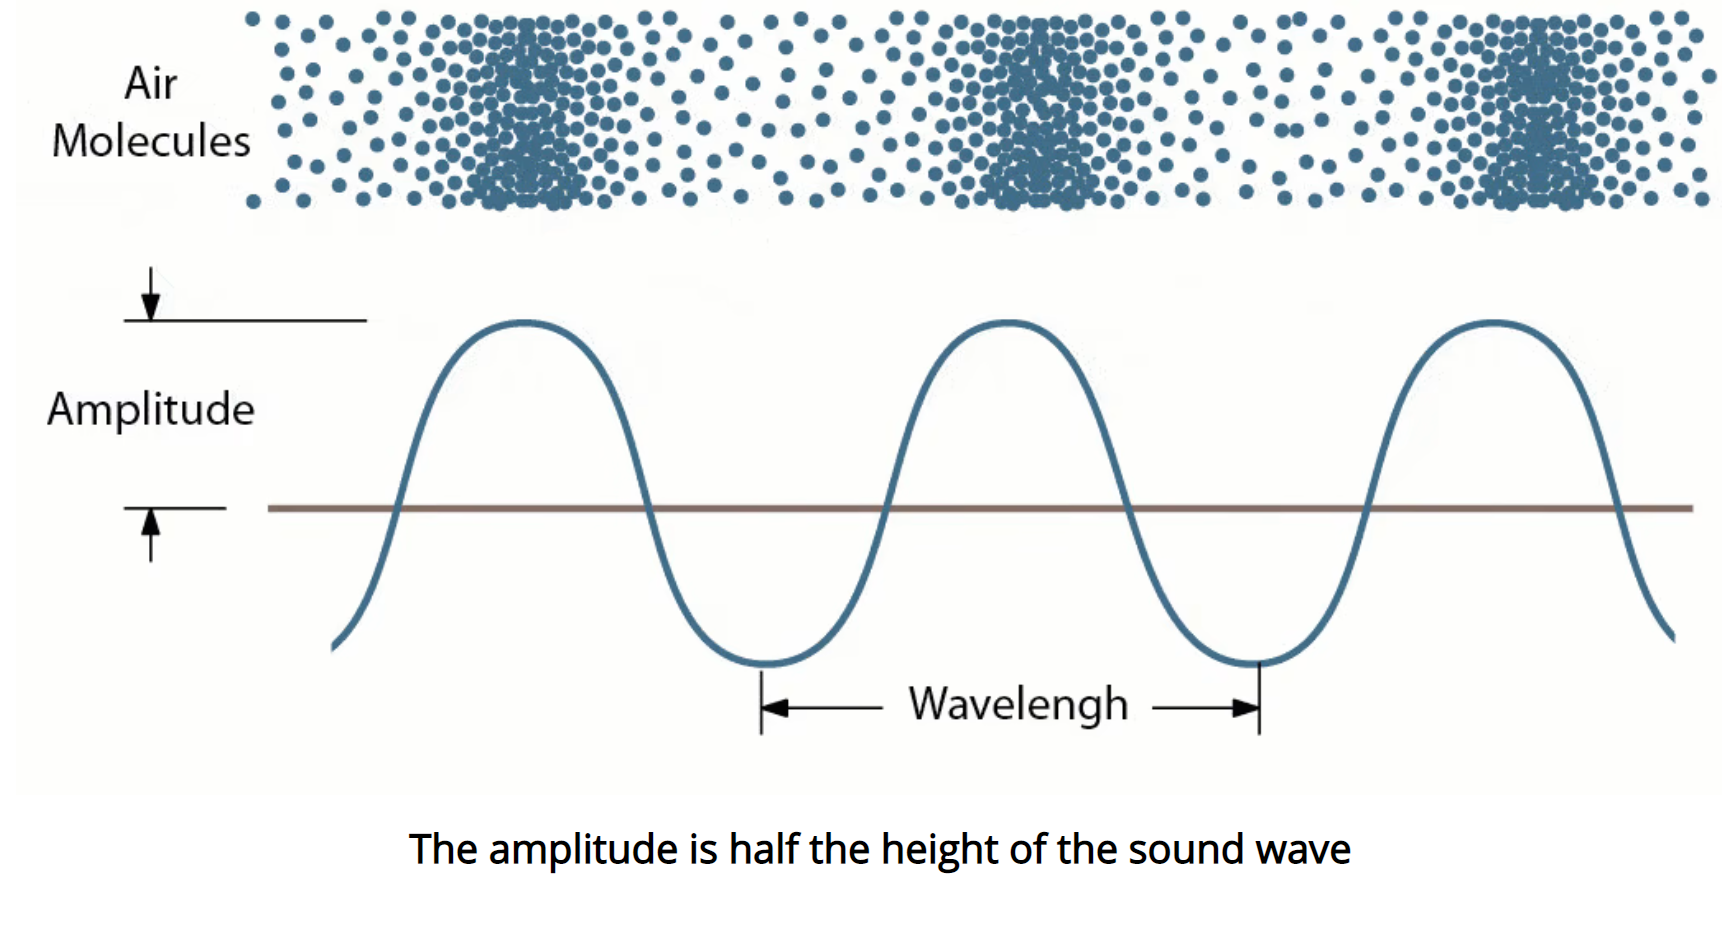
\includegraphics[width=0.70\textwidth]{graphics/soundwaves.png}
    \caption{How molecules react to sound waves \cite{noauthor_what_nodate}}
    \label{fig:SoundWaves}
\end{figure}

\subsubsection{Digital audio recording}

\fxfatal{Tala um jitter og kanski aliasing}

%https://documentation.meraki.com/MR/WiFi_Basics_and_Best_Practices/Signal-to-Noise_Ratio_(SNR)_and_Wireless_Signal_Strength#:~:text=The%20SNR%20is%20the%20difference,signal%20and%20the%20noise%20floor.&text=For%20example%2C%20if%20a%20client,dB%20for%20this%20wireless%20connection. - SNR

Audio recording is the recreation of sound waves, which can either be analog- or digital recorded.
Digital recording is the process of converting analog sounds, which can be convert the analog signals from a microphone to a digital format. 
Which is done by representing the audio signal with binary numbers 
This represents the amplitude or intensity of the sound and then sampling or recording that sound at a given time interval.
The greater the resolution the less noise is being recorded.
Resolution is determined by the number of bits used in order to record a signal and deter the precision of the measurements, it is the smallest incremental voltage change that can be recognized.
For example if a signal had a voltage range of 3.3V and it was being recorded at 16bits the voltage resolution would be $\frac{3.3V}{2^{16}} = 50\mu V/bit$.
Which would mean that the recording could in theory have $50\mu V$ increments in representing the signal.  
While a 8bit resolution only yields $\frac{13mV}{bit}$, meaning the higher the resolution, the more precise the measurement values are.
However with more bits comes more data rate and higher storage requirements.

\begin{equation}
    Data Rate = \frac{Bits}{8} * Sampling Rate * Number of channels 
    \label{eq:dataRate}
\end{equation}

Data rate can be calculated using \textit{Equation~\ref{eq:dataRate}}.
Where bits is the resolution, sampling rate is the sampling frequency in Hz and the number of channels is how many signals are being recorded.
The data rate can then be used to determine the amount of storage needed.
Nyquist-Shannon theorem is is in digital recording to determine the minimum sampling rate needed to reconstruct the analog signal.
The theorem proves that if the sampling frequency is twice the frequency of the highest frequency of the input analog signal, the signal can be recreated exactly.% \cite{bartlett_practical_2016}.
So in theory since humans have a hearing range of up to around 20kHz, in order to reconstruct all signals that are audible to humans, the sampling rate needs to be at least 40kHz.
For example on CDs the quality of the recording is 44.1kHz/16bits, in DVDs it is 96kHz/24bits and for high end audio recording it can go to 192kHz/24bits.
The oversampling can improve the recording for more accurate recording.
But oversampling is a term used for when the sampling frequency is of a higher rate than the Nyquist-Shannon theorem states  \cite{bartlett_practical_2016}.
If for example a sampling frequency of 200kHz was used when the signal being recorded was 20kHz it would be considered 5x oversampling. 
The difference in decibel between the signal and the noise floor is called signal to noise ratio (SNR). 
For cleaner sounds, meaning less noise is audible in the signal the higher the SNR.
Generally it is considered fair if the SNR is 60dB, good if SNR is 70dB and great if its 80dB or more.
\cite{bartlett_practical_2016}

\section{Device hardware}

\textbf{FARA 'I GEGNUM VERKEFNI SEM AÐRIR HAFA GERT RUNNA ÞAU OG TALA UM NIÐURSTÖÐUR OG DÆMA HVÐ VIRKAR HVAÐ EKKI OG AFHVERJU ÞETTA GETUR VERIÐ EH APPENDIX DÆMI
}

\subsection{Hydrophone}

Hydrophones are devices specially designed for underwater sound recording.
One of the earliest known examples of a hydrophone was made by stretching a membrane tightly over the end of a tube, one end of the tube is placed underwater while the other end is placed to the observers ear \cite{wood_a_b_textbook_1946}. 
Modern hydrophone are mainly based on piezoelectric transducers.
These hydrophones have been used since the early stages of world war 1.
Paul Langevin developed the first piezoelectric hydrophone, which was intended to be used for the detection of submarines.
A vacuum tube amplifier in combination with a piezoelectric material to be used as a transducer signal\cite{van_der_kloot_great_2014}.

When choosing a hydrophone it is important to look at a few specifications in the data sheet of the hydrophone. 
Such as the open circuit receiving response (OCRR), which is what the transducer outputs in terms of dB re 1V/$\mu$Pa.
Which is function of frequency and expressed in terms of dB re 1V/$\mu$Pa.
Sound intensity level (SIL) is the intensity of the sound at the transducer and is expressed in terms of dB re $\mu$Pa.
Transmitting voltage response (TVR) is the output voltage of the SIL at 1m range from the transducer and is expressed in terms of dB re $\mu$Pa/1V @ 1m \cite{ethem_mutlu_sozer_underwater_nodate}. 
Usable frequency of the hydrophone, directional patterns of the hydrophone and if the it applies the nominal capacitance of the hydrophone are also important factors. 
If for example the CRT C57 hydrophone was chosen, specifications can be seen in \textit{Table \ref{Tab:CRT57Hydrip}}.

\newpage

\begin{table}[h]\caption{Specifications of CRT C57 hydrophone range \cite{computing_c57_nodate}}.\label{Tab:CRT57Hydrip}
\centering
\begin{tabular}{|r|c|c|}
\hline
\multicolumn{1}{|c|}{\textbf{}} & C57 / C57X & C57RS/C57XRS \\\hline
{\begin{tabular}[c]{@{}r@{}}Linear Frequency Range \\ (±3dB) {[}kHz{]}\end{tabular}}      & 0.015 to 45         & \begin{tabular}[c]{@{}c@{}}0.015 to 50\&\\ 124 to 250+\end{tabular} \\ \hline
{\begin{tabular}[c]{@{}r@{}}Usable Frequency Range \\ (+3/-12dB) {[}kHz{]}\end{tabular}}  & 0.008 to 100        & { 0.008 to 77 \& 96 to 250+}                    \\ \hline
{\begin{tabular}[c]{@{}r@{}}Transducer Sensitivity* \\ {[}dB, re 1V/µPa{]}\end{tabular}}  & -187                & { -200}                                         \\ \hline
{Preamplifier Gain {[}dB{]}}                   & 20 / 33             & { 20 / 33}                                      \\ \hline
{\begin{tabular}[c]{@{}r@{}}Effective Sensitivity*\\  {[}dB, re 1V/µPa{]}\end{tabular}}   & -167 / -154         & { -180 / -167}  \\  \hline
\multicolumn{1}{|l|}{\begin{tabular}[c]{@{}l@{}}Price from dealer \\ {[}€{]}\end{tabular}} & \multicolumn{1}{|l|}{1290/1290} & \multicolumn{1}{|l|}{1290/1290} \\ \hline
\end{tabular}
\end{table}

If the CRT C57RS has an OCRR of -200 db re 1V/$\mu$Pa over a frequency range of 0.008 to 77kHz. 
Lets say a Blue whale is producing a moan which from \textit{Table \ref{Tab:WhaleHz}} indicates that the SIL would be 188dB re $\mu$Pa.
Then $VdB = SIL + OCRR = 188 + (-200) = -12dB$.
Because VdB is relative to 1V, the voltage output can be described as $V = 10^{VdB/10}$
which means the voltage output of the hydrophone would then be $V = 10^{-12dB/10} = 63mV$.

% Converting the oscillating mechanical pressure difference (sound waves) to electrical energy \cite{li_piezoelectric_2012}.
% https://www.researchgate.net/publication/255001750_Piezoelectric_Materials_Used_in_Underwater_Acoustic_Transducers
% https://archive.org/details/in.ernet.dli.2015.15768/page/n471/mode/2up
% https://en.wikipedia.org/wiki/Hydrophone#cite_note-3
%https://se.mathworks.com/help/phased/ref/phased.isotropichydrophone-system-object.html

\subsection{Signal conditioning}

Conditioning the output signal produced by the hydrophone is important in order to only monitor desired values.
Unwanted frequencies need to be filtered out in order to get a cleaner signal in the range that is desired.
In lower frequency application, from 0 - 100kHz a simple resistor and capacitor (RC) filters can generally be used \cite{noauthor_low_2013}.
High pass filters works by filtering out frequencies that are lower than the set cut off frequency ($F_c$) and allows frequencies higher to pass through.
The $F_C$ point is defined when the voltage output signal is 70.7\% of the input, which is when the output signal is -3dB that of the input.% = $20log(\frac{V_{out}}{V_{in}})$.
Low pass filters out higher frequencies than the set $F_c$ and allows frequencies that are lower to pass through. 
For first order filter this occurs at a rate of -20dB/Decade after the set $F_c$, the slope of which can be increased by increasing the order of the filter.
Examples of the RC filters can be seen in \textit{Figure \ref{fig:PassiveHighLow}}.
The $F_C$ point is defined when the output signal is 70.7\% of the input, which is when the the voltage gain is at -3dB = $20log(\frac{V_{out}}{V_{in}})$.

\begin{equation}
    F_c = \frac{1}{2\pi RC}
    \label{eq:FC}
\end{equation}

To find the cutoff frequency of a first order filter circuit \textit{Equation \ref{eq:FC}} can be used.
Where $R$ is the resistor value in $\Omega$ and $C$ is the capacitor value in farads $F$.
Since the filter contains a capacitor the output signal will lag behind the input signal and shifts phase compared to the input. 
The capacitor takes time to charge and causes a lag between the input and the output voltage \cite{noauthor_low_2013}. 

\begin{equation}
    \theta = \arctan(2 \pi fRC)
    \label{eq:phasshift}
\end{equation}

The phase shift angle can be found using \textit{Equation~\ref{eq:phasshift}}.
Where $\theta$ is the phase shift angle, f is the frequency of the input signal, R is the resistor value on $\Omega$ and C is the capacitor value in Farads $F$.

The time constant of the capacitor which is caused by the charging and discharging effects of the resistor and capacitor gives the circuit a response in the time domain. 
Which is the elapsed time for the circuit to respond to changes in the the input signal of the circuit.


\begin{equation}
    \tau = RC = \frac{1}{2\pi F_c}
    \label{eq:Tau}
\end{equation}

The time constant of the RC filters can be found using \textit{Equation~\ref{eq:Tau}}. 
Where $\tau$ is the time constant,R is the resistor value on $\Omega$ and C is the capacitor value in Farads $F$ and $F_c$ is the cutoff frequency. 

\begin{figure}[h]
    \centering
    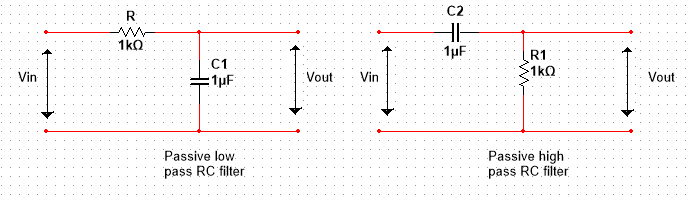
\includegraphics[width=0.70\textwidth]{graphics/passivehighlow.png}
    \caption{Passive low and high pass filters RC filter setups.}
    \label{fig:PassiveHighLow}
\end{figure}

Operational amplifiers or op amps are device that amplify voltage signals.
These devices are heavily used in signal conditioning and filtering.
The DC gains of op amps is a ratio between the input voltage and the output voltage. 

\begin{equation}
    A_v = \frac{V{out}}{V{in}} = 1 + \frac{R_f}{R_{in}}
    \label{eq:DCGain}
\end{equation}

The gain from a non inverting op amp can be found by \textit{Equation \ref{eq:DCGain}}, $A_v$ is the gain and $R_f$ and $R_{in}$ are the resistor values of the resistor configuration seen on the left hand side in \textit{Figure \ref{fig:invNonInvOPamp}}.


\begin{equation}
    A_v = -\frac{V{out}}{V{in}} = -\frac{R_f}{R_{in}}
    \label{eq:invertDCGain}
\end{equation}

The gain from a inverting op amp can be found by \textit{Equation \ref{eq:invertDCGain}}, $A_v$ is the gain and $R_f$ and $R_{in}$ are the resistor values of the resistor configuration seen on the right hand side in \textit{Figure \ref{fig:invNonInvOPamp}}.

\begin{figure}[h]
    \centering
    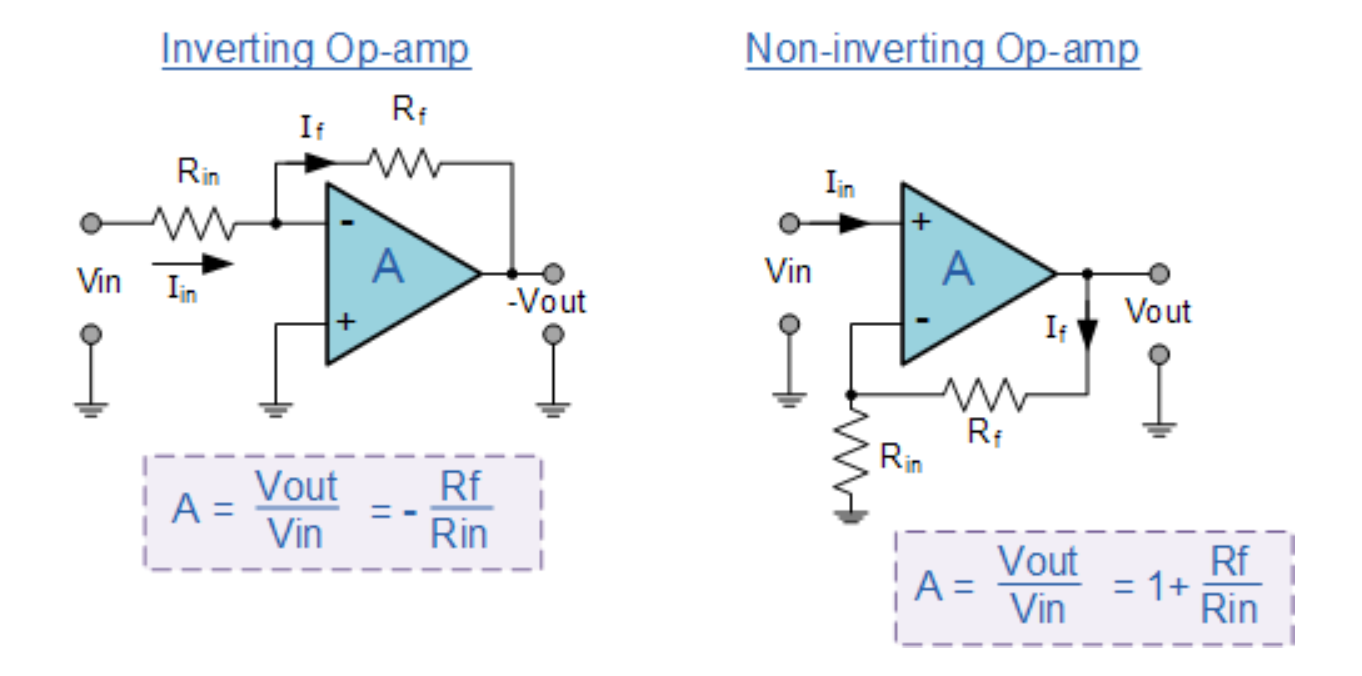
\includegraphics[width=0.70\textwidth]{graphics/invNoninv.png}
    \caption{Inverting and non inverting op amp setups \cite{noauthor_operational_2013}.}
    \label{fig:invNonInvOPamp}
\end{figure}

When the RC filter and op amps are combined, they form what is called an active filter.
Examples of which can be seen in \textit{Figures \ref{fig:LowPassFilter},\ref{fig:HighPassFiler}} and their respective frequency and phase shift responses in \textit{Figures \ref{fig:LowPassResponse},\ref{fig:HighPassResponse}}.
These filters performs the same as an RC filter in terms of its operations and frequency response with the addition of gain control \cite{noauthor_active_2013-1}.


\begin{equation}
    A_f = \frac{V{out}}{V{in}} = \frac{A_v}{\sqrt{1 + (\frac{f}{f_c})^2}}
    \label{eq:ActiveLowPass}
\end{equation}





The gain of the first order active low pass filter can be found using \textit{Equation \ref{eq:ActiveLowPass}}.
Where $A_f$ is the voltage gain, $A_v$ is the dc gain seen in \textit{Equation \ref{eq:DCGain}}, f is the frequency of the signal and $F_c$ is the set cutoff frequency.
This has the effect of active gain control depending on the frequency of the input.
When,
\begin{enumerate}
    \item $f < F_c$, $A_f \approx A_v$
    \item $f = F_c$, $A_f = \frac{A_v}{\sqrt{2}} = 0.707 A_v$
    \item$f > F_c$, $A_f < A_v$
\end{enumerate}

\begin{figure}[h]
    \centering
    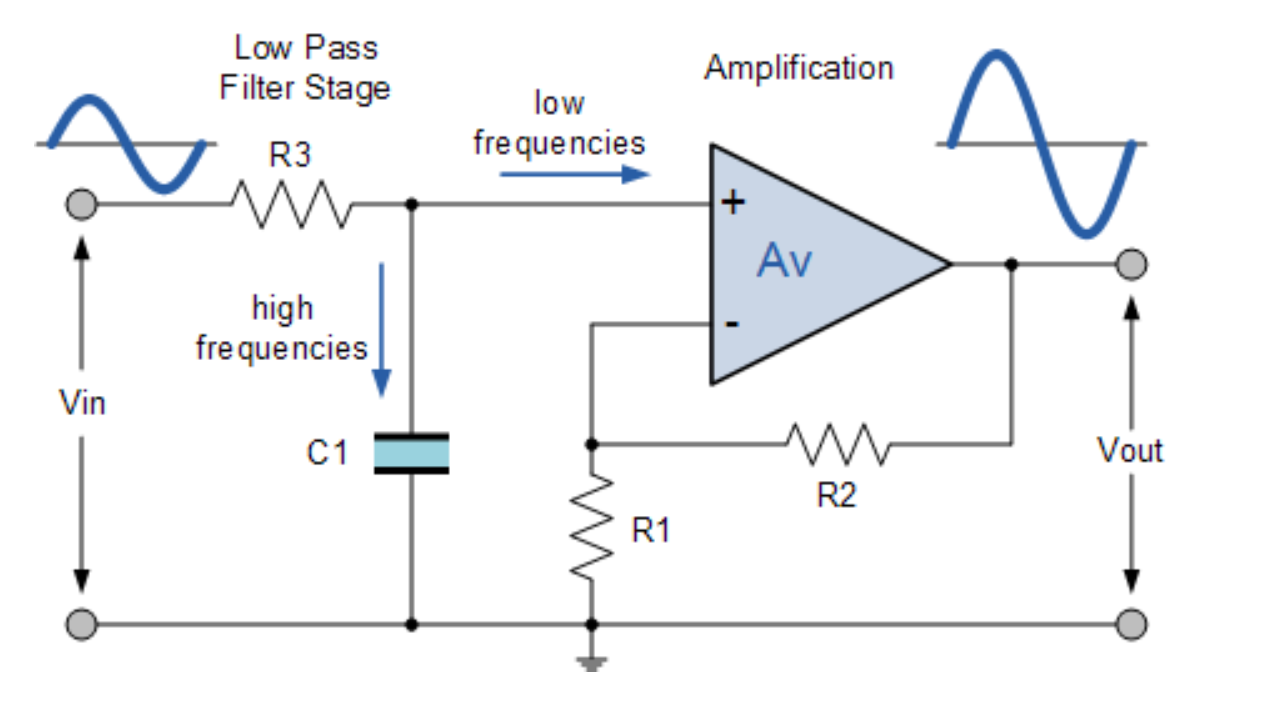
\includegraphics[width=0.70\textwidth]{graphics/lowPassFilter.png}
    \caption{Active first order low pass filter \cite{noauthor_active_2013-1}.}
    \label{fig:LowPassFilter}
\end{figure}

\begin{figure}[h]
    \centering
    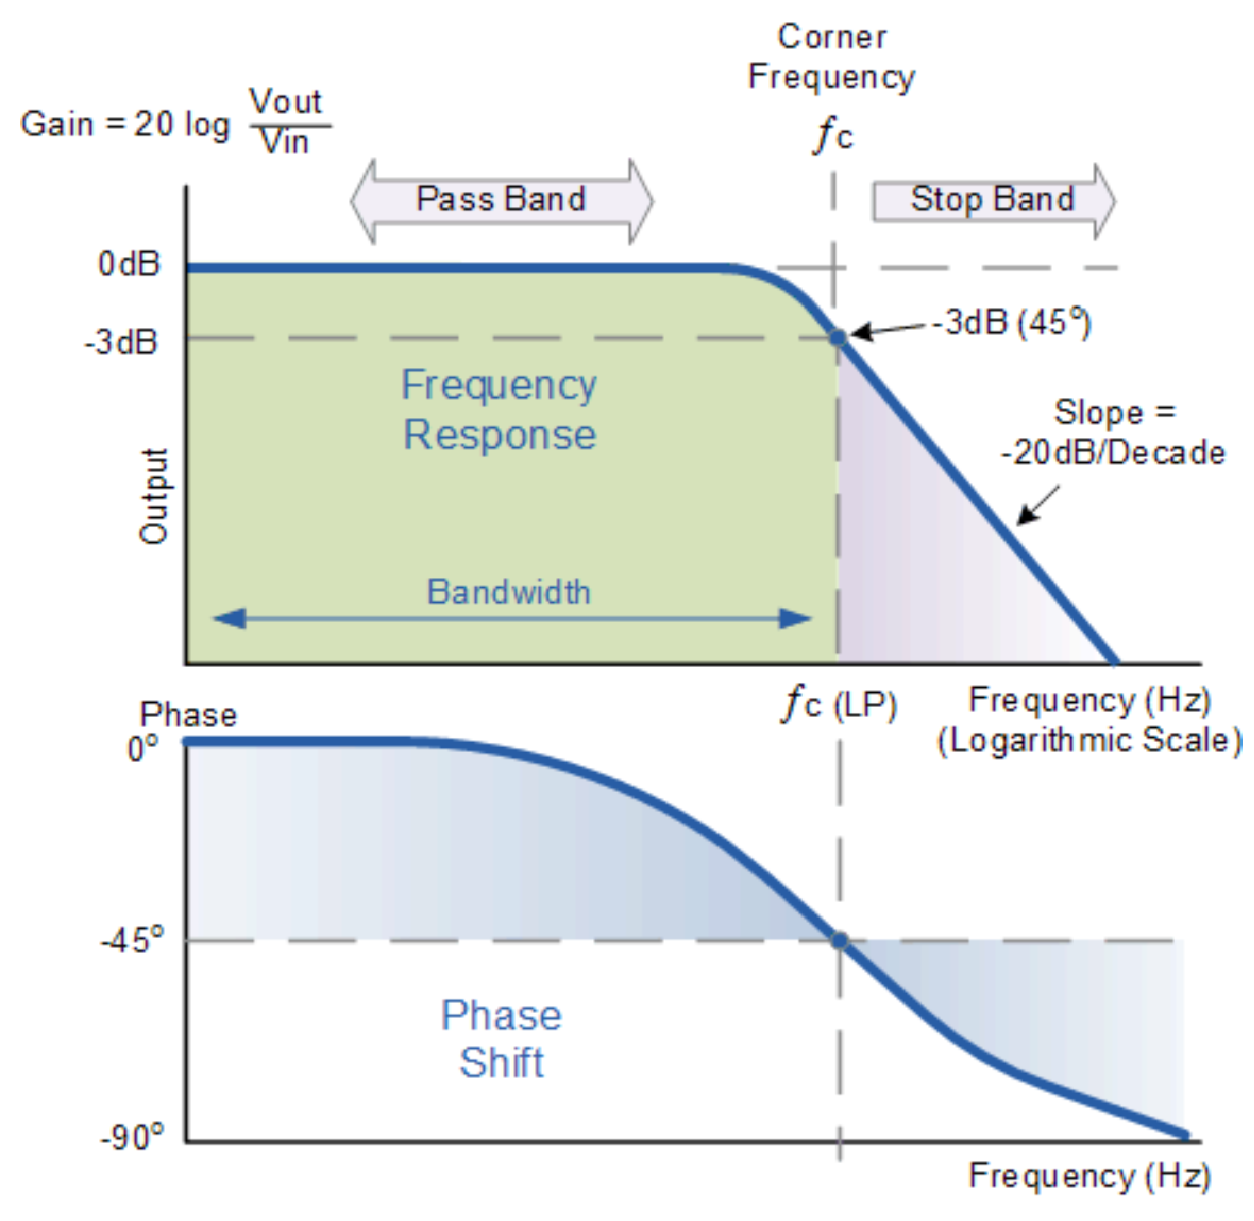
\includegraphics[width=0.70\textwidth]{graphics/lowPassResponse.png}
    \caption{First order RC low pass frequency response and phase shift \cite{noauthor_low_2013}}
    \label{fig:LowPassResponse}
\end{figure}

\begin{equation}
    A_f = \frac{V{out}}{V{in}} = \frac{A_v(\frac{f}{f_c})}{\sqrt{1 + (\frac{f}{f_c})^2}}
    \label{eq:ActiveHighPass}
\end{equation}

The gain of the first order active high pass filter can be found using \textit{Equation \ref{eq:ActiveHighPass}}.
Where $A_f$ is the voltage gain, $A_v$ is the dc gain seen in \textit{Equation \ref{eq:DCGain}}, f is the frequency of the signal and $F_c$ is the set cutoff frequency.
This has the effect of active gain control depending on the frequency of the input.
When,
\begin{enumerate}
    \item $f < F_c$, $A_f < A_v$
    \item $f = F_c$, $A_f = \frac{A_v}{\sqrt{2}} = 0.707 A_v$
    \item$f > F_c$, $A_f \approx A_v$
\end{enumerate}


\begin{figure}[h]
    \centering
    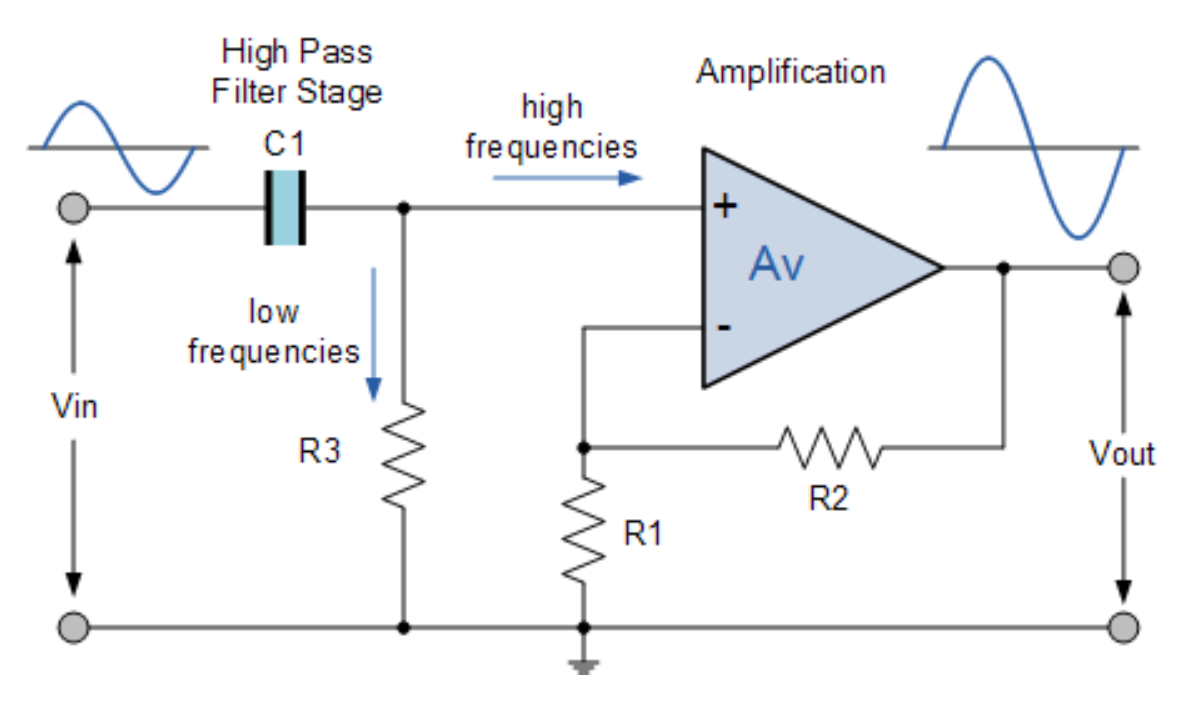
\includegraphics[width=0.60\textwidth]{graphics/highPassFilter.png}
    \caption{Active first order low pass filter \cite{noauthor_active_2013}.}
    \label{fig:HighPassFiler}
\end{figure}

\begin{figure}[h]
    \centering
    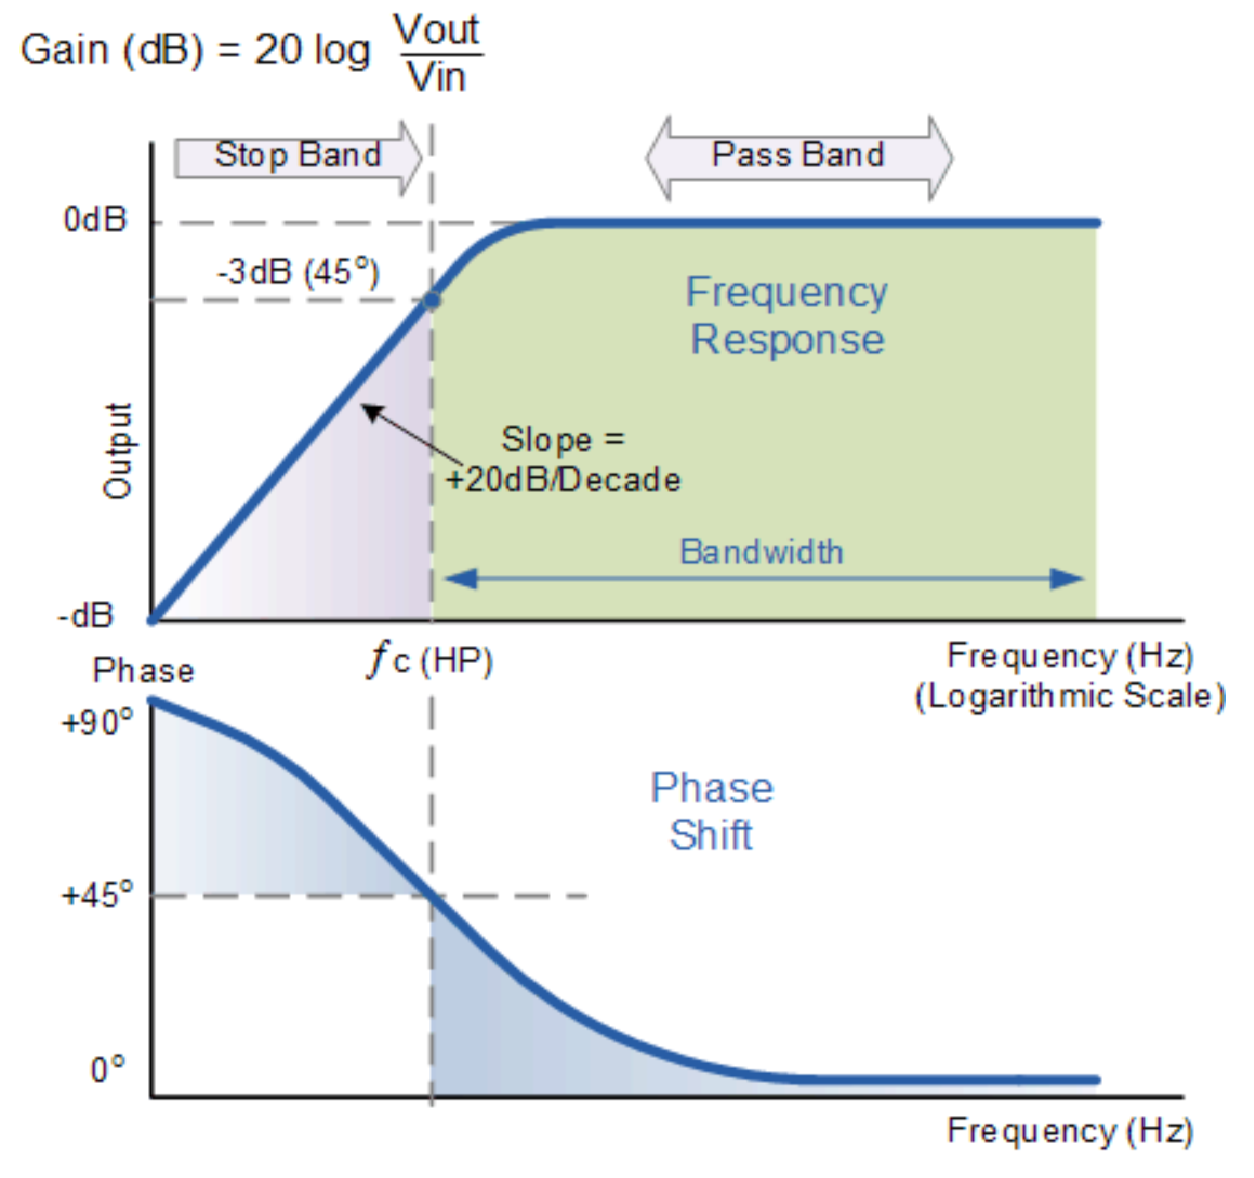
\includegraphics[width=0.60\textwidth]{graphics/highPassResponse.png}
    \caption{First order RC high pass frequency response and phase shift \cite{noauthor_high_2013}}
    \label{fig:HighPassResponse}
\end{figure}

\clearpage

Decibel is a relative unit of measure, used in electronic circuit to express ratio of input values to output value on a logarithmic scale.  

\begin{equation}
    dB = 20log\frac{V{out}}{V{in}}
    \label{eq:DBGAIN}
\end{equation}

The gain in decibel is found by \textit{Equation \ref{eq:DBGAIN}}, where $V{out}$ is the output root mean square (rms) voltage of the circuit and V{in} is the input rms voltage.

Summing amplifiers or summing inverter circuits are useful when combining two or more signals together.
An example of the circuit can be seen in \textit{Figure \ref{fig:SummingOpAmp}}, where $R_1 = R_2 = R_3$ would be the same value.
The circuit yields a voltage output that is equal to all the input voltages summed together, multiplied with the unity gain of the amplifier.
This is possible due to the virtual ground that is created by a non inverting op amp configuration\cite{noauthor_summing_2013}. 
This circuit is especially useful when there is a need to shift the signal from an oscillating AC voltage to an oscillating DC voltage.


\begin{figure}[h]
    \centering
    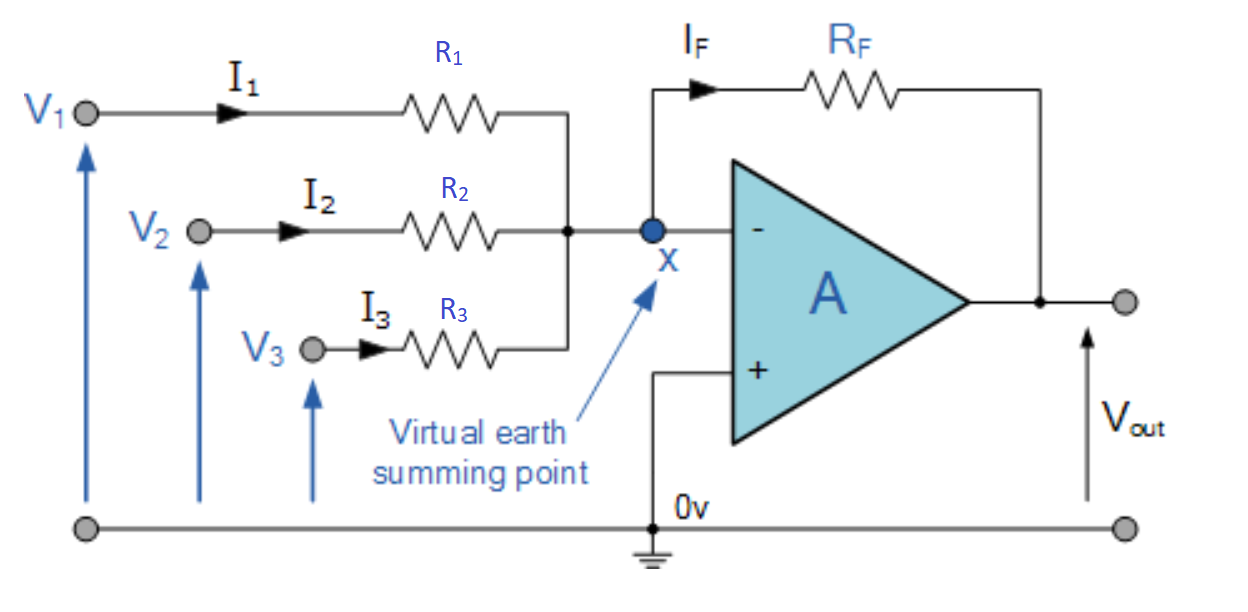
\includegraphics[width=0.70\textwidth]{graphics/SummingOpAmp.png}
    \caption{Scaling summing amplifier circuit \cite{noauthor_summing_2013}}
    \label{fig:SummingOpAmp}
\end{figure}


\begin{equation}
    I_F = I_1 + I_2 + I_3 = -[\frac{V_1}{R_{1}} + \frac{V_2}{R_{2}} + \frac{V_3}{R_{3}}]
\end{equation}


$$-V_{out} = \frac{R_F}{R_{1}}V_1 +\frac{R_F}{R_{2}}V_2 +\frac{R_F}{R_{3}}V_3$$

Scaling summing amplifiers are in the same configuration as summing amplifiers with one main difference which is that resistor values are not equal to one another.
This enables individual scaling of each signal, which means that each input signal can have different gain values.

\begin{equation}
    V_{out} = -R_F(\frac{V_1}{R_{1}} +\frac{V_2}{R_{2}} +\frac{V_3}{R_{3}} + ...)
    \label{eq:ScalingGain}
\end{equation}

Finding the output voltage can be found using \textit{Equation \ref{eq:ScalingGain}}.
Where $V_out$ is the output voltage, $R_f$ is the voltage across the input and output of the op amp, $R_1, R_2$ and $R_3$ are the resistor value of the different input signals.
Lets take for an example of an AC signal that needs to be shifted so that there is no negative voltage, see \textit{Figure \ref{fig:sumCircuitexamp}} for the layout of the circuit.
The AC signal (U1B\_out) would along with the shifting signal, in this case a DC voltage of 1.65V.
The AC signal is scaled by a factor of A = $\frac{180\Omega}{90\Omega}$ = 2.
How ever the DC voltage signal only scaled by a factor of A = $\frac{180\Omega}{180\Omega}$ = 1.
The voltage output, U1C\_out can be seen in \textit{Figure \ref{fig:SummingOpAmpShift}} as the red signal and the input signal, U1B\_out is represented by the white signal.
This creates a problem though, the output signal is shifted by $90\deg$ and the scaling op amp is in a inverting configuration the signal is inverted, so it is negative.
Both are fixed by the addition of U1D, an inverting amplifier.
Which puts the signal back in phase with the original input signal as well as it now is positive, as seen in \textit{Figure \ref{fig:SummingOpAmpShift1}} where the red signal is U1D\_out the output of the inverting amplifier and the white signal is the original input signal U1B\_out.


\begin{figure}[h]
    \centering
    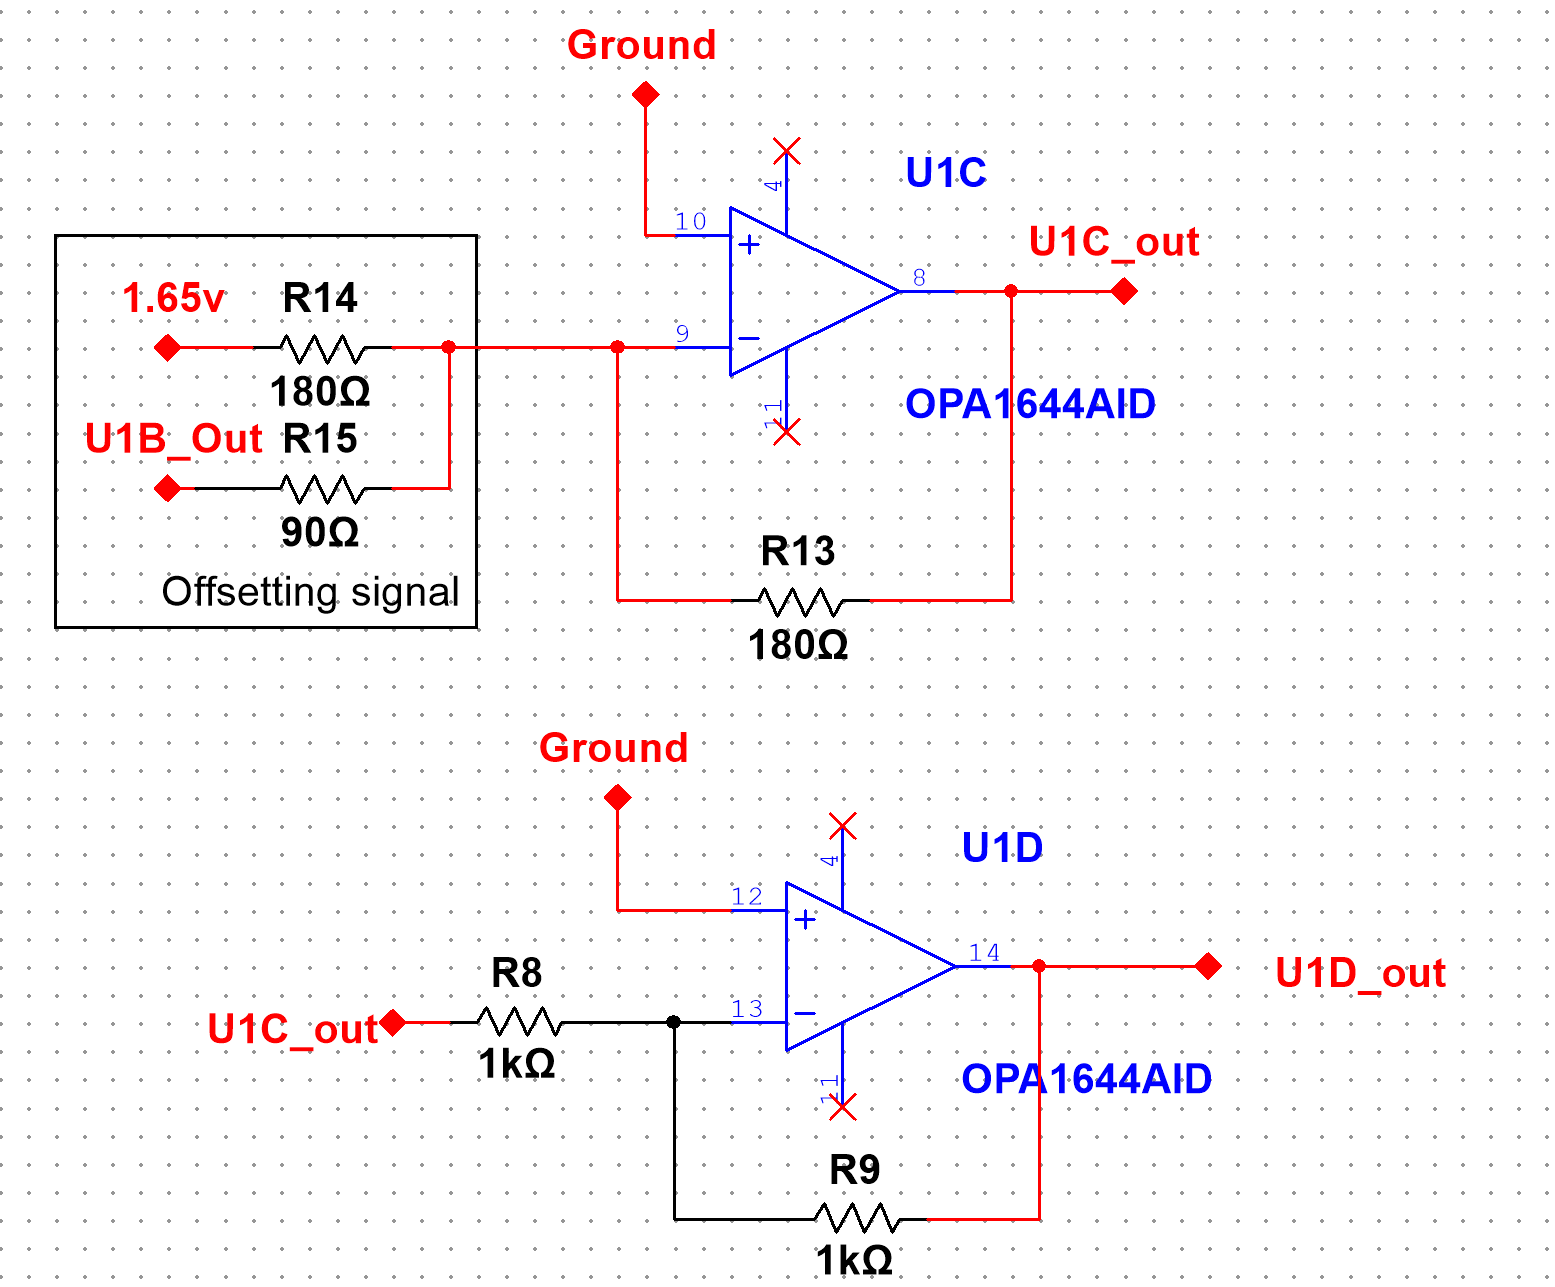
\includegraphics[width=0.70\textwidth]{graphics/sumCircuitexamp.png}
    \caption{Example of a scaling amplifier circuit where two signals are combined to create a shift of the original signal. U1C represents the scaling amplifier, U1D is a normal inverting amplifier.}
    \label{fig:sumCircuitexamp}
\end{figure}

\begin{figure}[h]
    \centering
    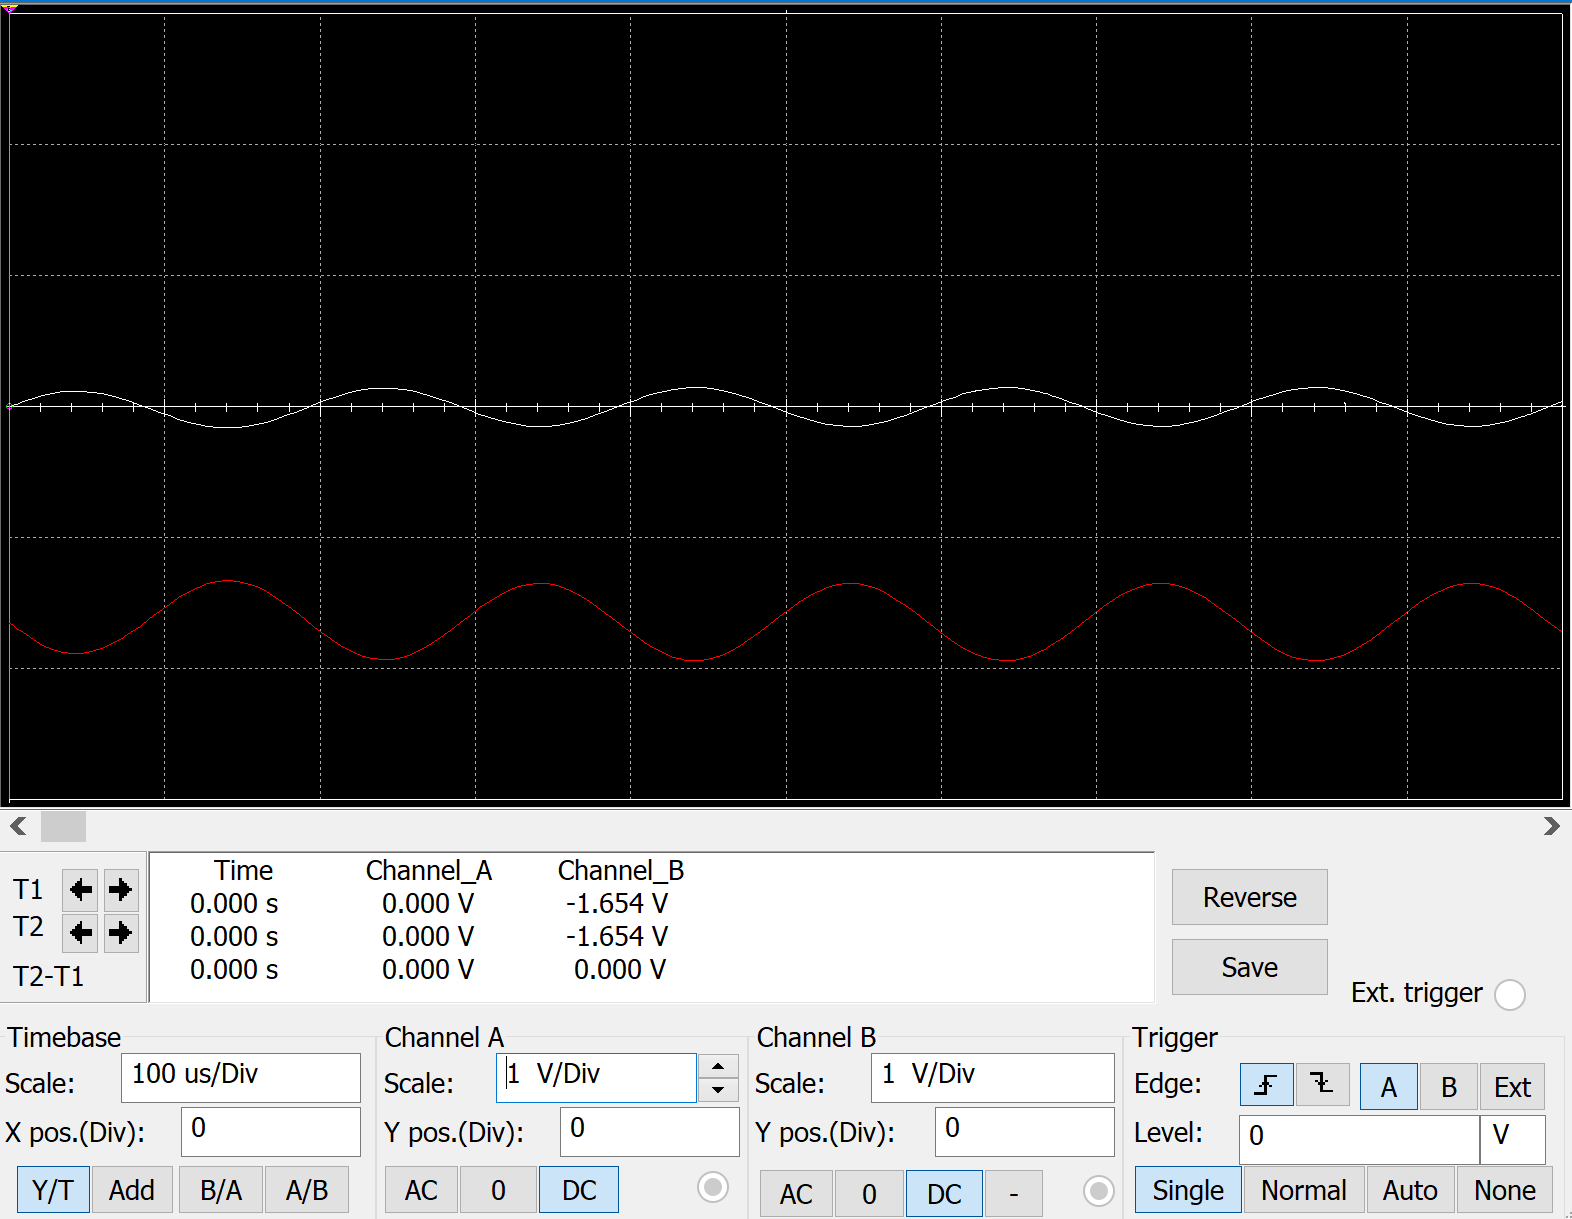
\includegraphics[width=0.70\textwidth]{graphics/summingShift.png}
    \caption{Example of the signal shift of a summing Op Amp circuit, the red signal represents the voltage output U1C\_out and the white signal is the input AC signal U1B\_out.}
    \label{fig:SummingOpAmpShift}
\end{figure}

\begin{figure}[h]
    \centering
    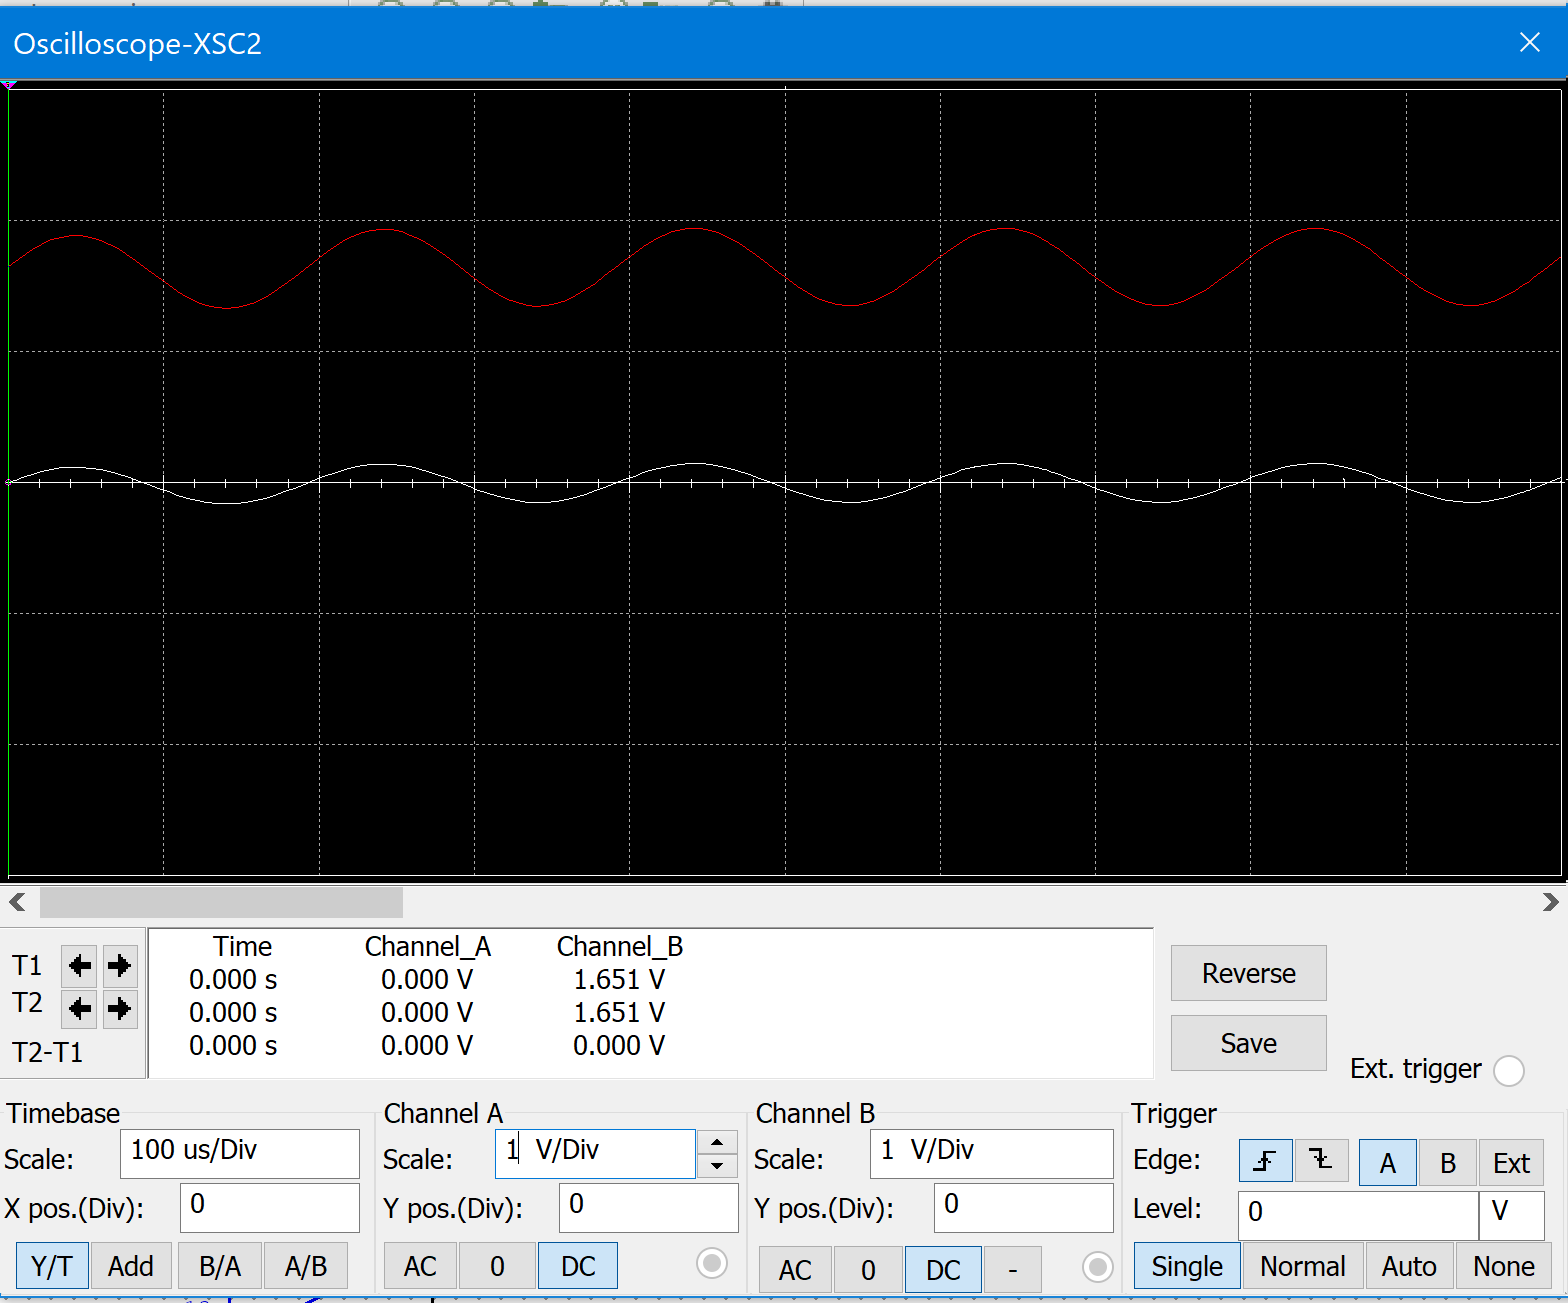
\includegraphics[width=0.70\textwidth]{graphics/summingShift1.png}
    \caption{Example of the signal shift of a summing Op Amp circuit, the red signal represents the voltage output U1D\_out and the white signal is the input AC signal U1B\_out}
    \label{fig:SummingOpAmpShift1}
\end{figure}


\clearpage

\fxfatal{SKOÐA H'ER-----------------------}
%ADC CHARECTERISTICS https://forum.pjrc.com/threads/44929-Teensy-3-5-ADC-characteristcs
%SD POSSIBLE https://forum.pjrc.com/threads/45993-Teensy-3-6-ADC-DMA-Question
%Teensy36ISRLogger Skilar með 8gb kortinu 6.67MB/s
%https://forum.pjrc.com/threads/49975-writing-binary-file-on-SD-card-in-Teency-3-5

\subsection{Microcontroller/Microcomputer}%Breyta um titil

For this project the most important factors when choosing a microcontroller/microcomputer were regarding the ADC specifications as well as the power consumption.\textbf{VITNA Í GOALS} tala um upplausn bit, power og fleira

\subsubsection{Arduino}

Arduino Uno is a programmable board that uses the 8-bit ATmega328p microcontroller.
Which is probably one of the most popular microcontroller in the world and the Arduino board is one of the among the best beginner boards to use because of the shear amount of documentation and tutorials for it.
The microcontroller main features can be seen in \textit{Table \ref{Tab:ATmega328p}}.


\begin{figure}[h]
    \centering
    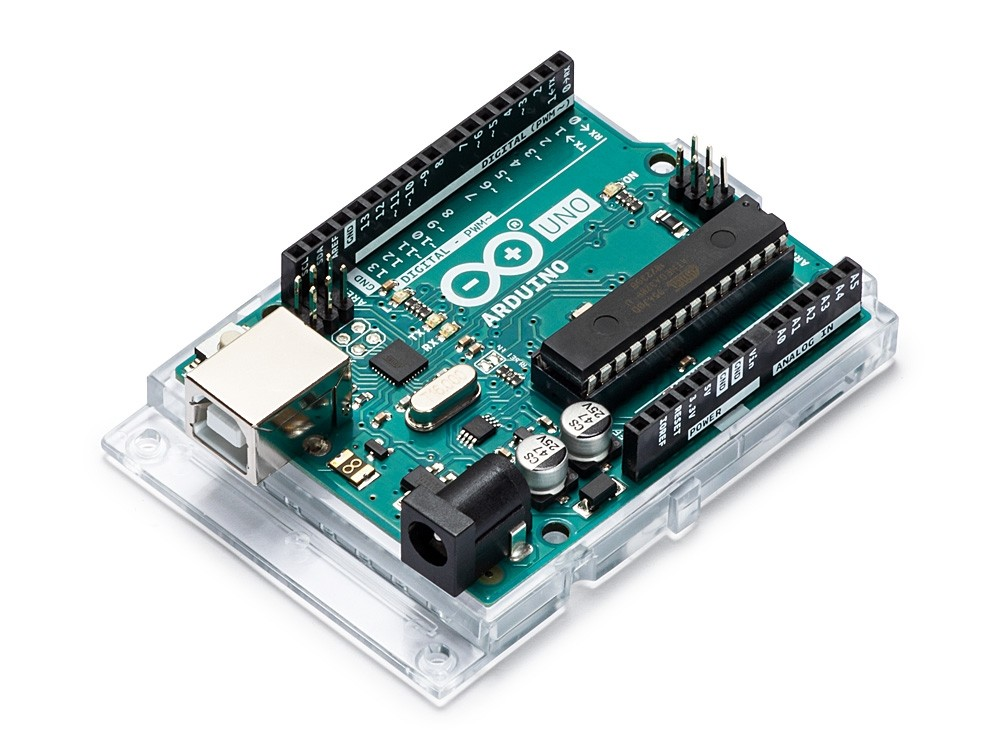
\includegraphics[width=0.70\textwidth]{graphics/ArduinoUNo.jpg}
    \caption{The Arduino Uno \cite{noauthor_arduino_nodate}}
    \label{fig:Arduino}
\end{figure}

\begin{table}[h]\caption{Main features of the ATmega328p \cite{noauthor_atmega328p_nodate}}.\label{Tab:ATmega328p}
\centering
    \begin{tabular}{|l|l|}
    \hline
        Parameters                        & Value                \\ \hline
        Flash memory [KB]                 & 32                      \\ \hline
        ADC resolution [bit]              & 10                   \\ \hline
        ADC sample speed [ksps]           & 15                     \\ \hline
        Digital Communication Peripherals & 1-UART, 2-SPI, 1-I2C \\ \hline
        Operating Voltage [V]             & 1.8 to 5.5           \\ \hline
        Max power consumption [W]         & 0.66               \\ \hline
        Price                             & 33\$                \\ \hline
    \end{tabular}
\end{table}


The Arduino has 14 digital input/output (I/O), and 6 can be used as pulse width modulation (PWM) outputs as well as 6 analog inputs.
The board has a USB connector which the board is programmed through as well as power it.
Arduino also provides its users with a free open source Arduino software integrated development environment (IDE).  \cite{noauthor_arduino_nodate}.
As well as a 6-channel 10-bit resolution ADC, with a conversion time of 65 to 260 $\mu s$ and up to 15 kilo samples per second (ksps) .
The board has a maximum current draw of 200mA, so at a operating voltage of 3.3V the power consumption is maximum 0.66W\cite{noauthor_atmega328p_nodate}.

%\textit{ It has 14 digital input/output pins (of which 6 can be used as PWM outputs), 6 analog inputs, a 16 MHz ceramic resonator (CSTCE16M0V53-R0), a USB connection, a power jack, an ICSP header and a reset button. It contains everything needed to support the microcontroller; simply connect it to a computer with a USB cable or power it with a AC-to-DC adapter or battery to get started.. You can tinker with your Uno without worrying too much about doing something wrong, worst case scenario you can replace the chip for a few dollars and start over again. "Uno" means one in Italian and was chosen to mark the release of Arduino Software (IDE) 1.0. The Uno board and version 1.0 of Arduino Software (IDE) were the reference versions of Arduino, now evolved to newer releases. The Uno board is the first in a series of USB Arduino boards, and the reference model for the Arduino platform; for an extensive list of current, past or outdated boards see the Arduino index of boards.}\cite{noauthor_arduino_nodate}.


\subsubsection{Raspberry Pi}

Unlike the Arduino the Raspberry Pi is not only a programmable microcontroller, but rather a single board microcomputer and is the third most sold computer brand worldwide \cite{noauthor_faqs_nodate}.
Currently there are 13 different model of the Raspberry Pi's with varying pricing and capabilities  some of which can be seen in \textit{Table \ref{Tab:RaspbModel}}. 
Raspberry Pis can be used with several operating system, for instance Linux, FreeBSD or a Raspberry pi OS that can come with or without a desktop.

\begin{center}
\begin{table}[h]\caption{Comparison of different Raspberry Pi models\cite{noauthor_faqs_nodate}}.\label{Tab:RaspbModel}
    \begin{tabular}{|l|l|l|l|c|}
    \hline
    \textbf{\begin{tabular}[c]{@{}l@{}}Raspberry Pi\\ Product\end{tabular}}        & \textbf{SoC} & \textbf{Speed} &  \textbf{\begin{tabular}[c]{@{}l@{}}Recommended\\ power supply \\ current capacity\end{tabular}} & \textbf{\begin{tabular}[c]{@{}l@{}}Typical bare-\\board current \\ consumption\end{tabular}} \\ \hline
     Model A+   & BCM2835      & 700MHz         & 0.7A          & 0.2A            \\ \hline
     Model B+   & BCM2835      & 700MHz         & 1.8A          & 0.33A            \\ \hline
     2 Model B  & BCM2836/7    & 900MHz         & 1.8A          & 0.5A                 \\ \hline
     3 Model B  & BCM2837A0/B0 & 1200MHz        & 2.5A          & 0.4A                  \\ \hline
     3 Model A+ & BCM2837B0    & 1400MHz        & 2.5A          & 0.35A                  \\ \hline
     3 Model B+ & BCM2837B0    & 1400MHz        & 2.5A          & 0.5A                  \\ \hline
     4 Model B  & BCM2711      & 1500MHz        & 3.0A          & 0.6A                  \\ \hline
     Zero       & BCM2835      & 1000MHz        & 1.2A          & 0.1A                   \\ \hline
     Zero W     & BCM2835      & 1000MHz        & 1.2A          & 0.15                  \\ \hline
     Zero WH    & BCM2835      & 1000MHz        & 1.2A          & 0.15                  \\ \hline
     400        & BCM2711      & 1800MHz        & 3.0A          & 0.8A                  \\ \hline
    \end{tabular}
\end{table}
\end{center}

Raspberry recommends powering the Raspberry Pi using 5V.
This means that the Raspberry Pi uses quite a bit of power,Raspberry Pi Zero (6W) Raspberry Pi 2 B (9W), Raspberry Pi 3(12.5W).
Taking a closer look at the Raspberry Pi Zero since it fits within the power consumption specifications.
The microcomputer costs around 30 \$, has a 1GHz single-core CPU, 512MB RAM, Mini HDMI port, Micro USB OTG port,
Micro USB power and HAT-compatible 40-pin header.
It has i2c, SPI, PWM and serial pins, all GPIO pins are digital and can be configured to be input or output pins.
which can be seen in \textit{Figure \ref{fig:RPIGPIO}}.

\begin{figure}[h]
    \centering
    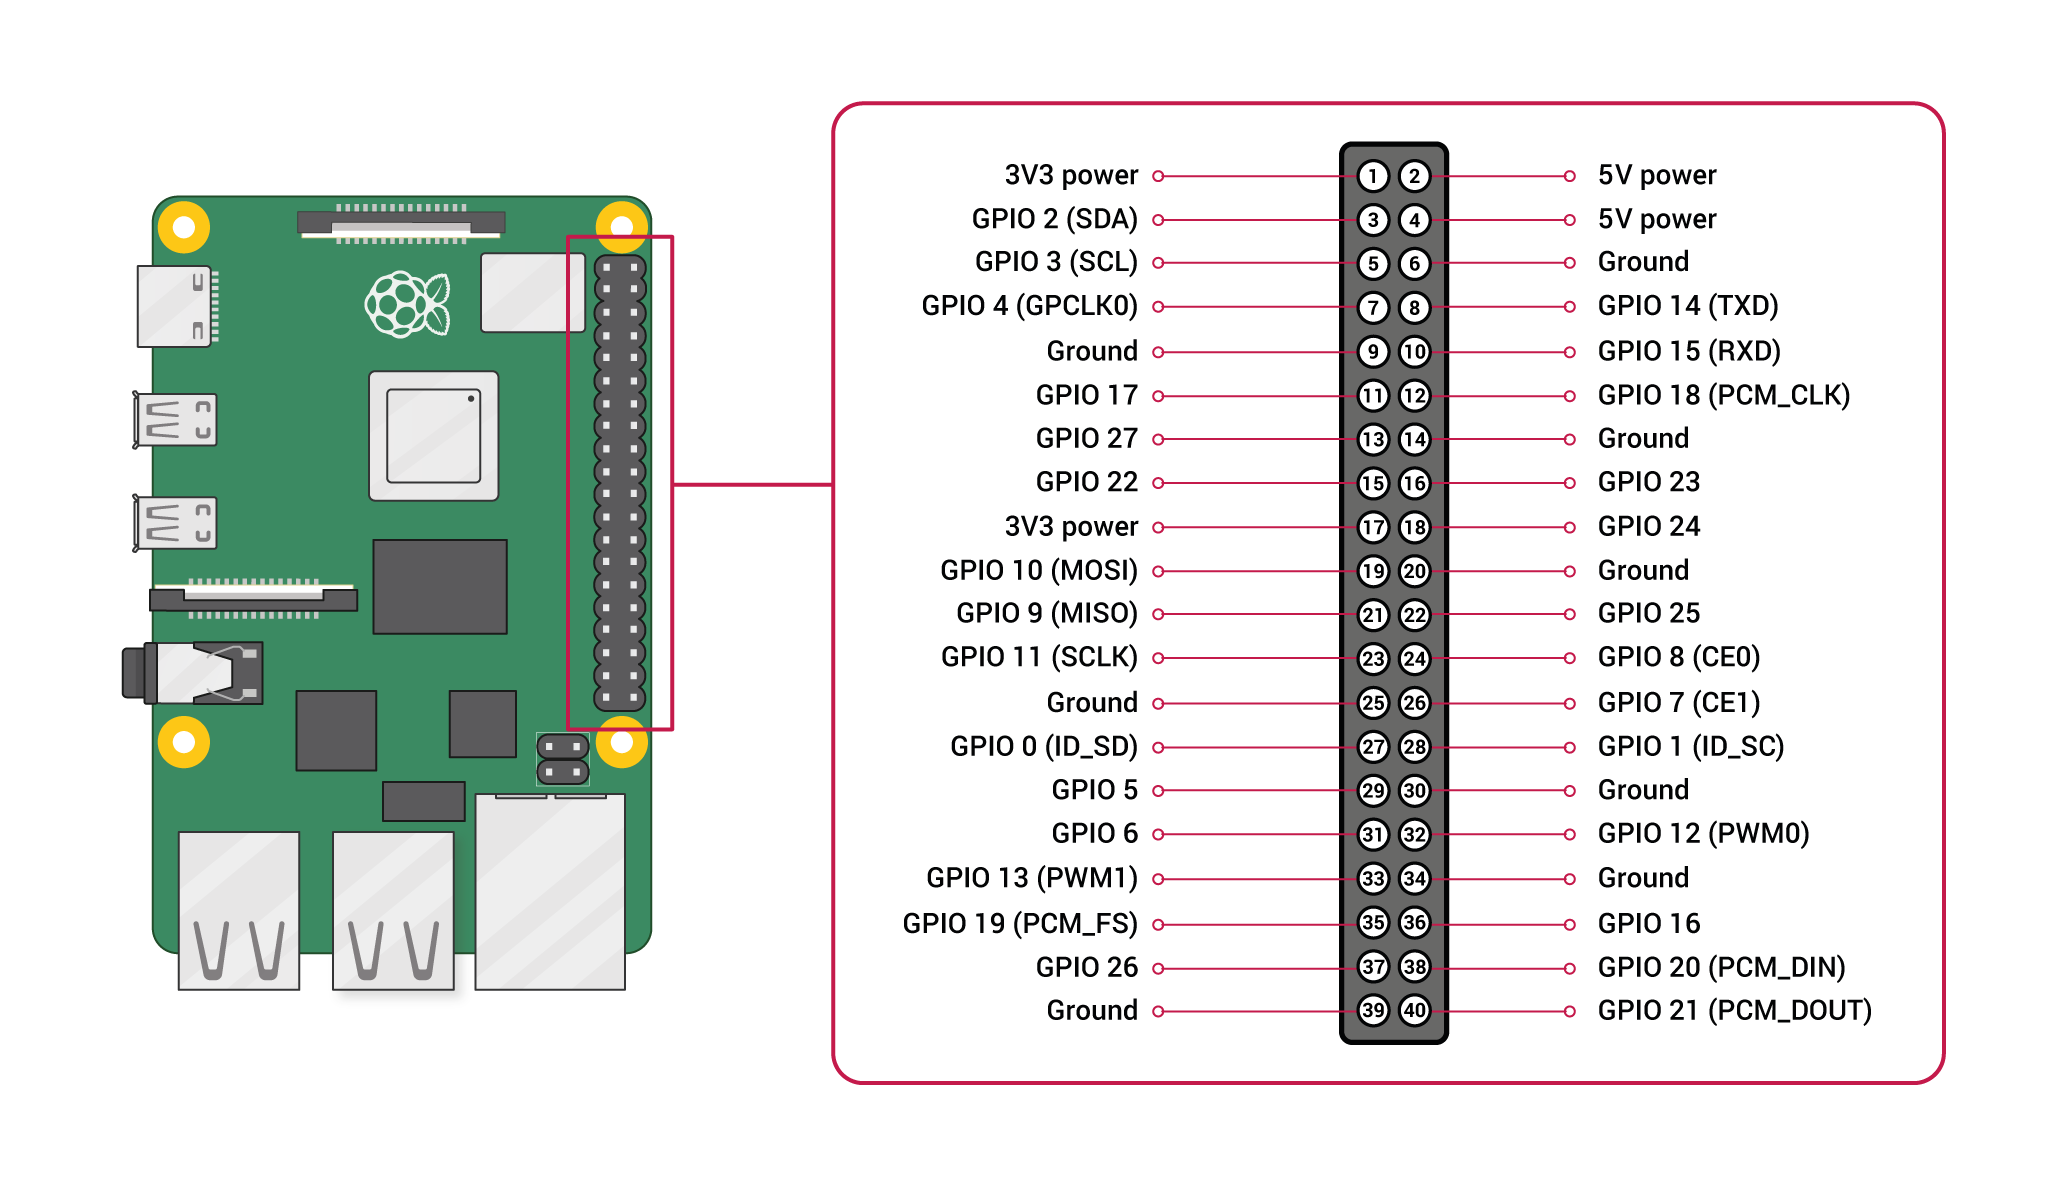
\includegraphics[width=0.70\textwidth]{graphics/ZeroGPIO.png}
    \caption{GPIO of the Raspberry Pi Zero \cite{noauthor_gpio_nodate}}
    \label{fig:RPIGPIO}
\end{figure}

The Raspberry Pi is however limited in the fact that it has no analog I/O pins, meaning that it can not convert analog to digital signal on its own.
However there is a way to record audio, which is done through sound card.
Several solutions have already been made available for this such as the Audio Injector stereo sound card which can directly connect to the general purpose input output (GPIO) pins of Raspberry Pi2, Pi3 and Pi Zero.
The card is made for an electret microphone and can supply the Raspberries with input and output audio.
The card has stereo RCA input and output, a headphone jack and a preamplifier, a volume knob and a low latency of 540 $\mu$s for both the input and output \cite{noauthor_rpi_nodate}.

\begin{figure}[h]
    \centering
    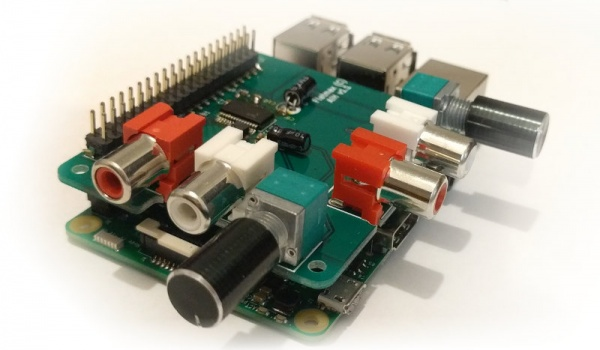
\includegraphics[width=0.70\textwidth]{graphics/rpisoundcard.jpg}
    \caption{The Audio Injector stereo sound card \cite{noauthor_rpi_nodate}}
    \label{fig:rpisoundcard}
\end{figure}


\subsubsection{Teensy}

Teensy's are the same as Arduino as being a USB programmable single board microcontroller.
The boards are can be programmed with multiple of programs such as the Arduino IDE software and can use both the examples and libraries that come with the program.
This is possible through an addition called Teensyduino which allso includes a large library for programing.
Other programs include Visual Micro, which enables programming on Visual Studio Code, PlaformIO IDE and CircuitPython (only available on Teensy 4.X) which allows python programming.
There are multiple models available, ranging in price, size and capabilities as seen in \textit{Table \ref{Tab:TeensyModel}}.


\begin{table}[h]\caption{Comparison of different Teensy models\cite{noauthor_teensy_nodate}}.\label{Tab:TeensyModel}
\begin{tabular}{|l|l|l|l|l|}
\hline
\multicolumn{1}{|c|}{\textbf{Specification}} & \multicolumn{1}{c|}{\textbf{Teensy 2.0}}                               & \multicolumn{1}{c|}{\textbf{Teensy 3.0}}                                            & \multicolumn{1}{c|}{\textbf{Teensy 3.5}}                                                  & \multicolumn{1}{c|}{\textbf{Teensy 4.1}}                                              \\ \hline
Processor & \begin{tabular}[c]{@{}l@{}}ATMEGA32U4\\ 8 bit AVR\\ 16 MHz\end{tabular} & \begin{tabular}[c]{@{}l@{}}MK20DX128\\ 32 bit ARM\\ Cortex-M4\\ 48 MHz\end{tabular} & \begin{tabular}[c]{@{}l@{}}MK64FX51\\2VMD12\\ 32-bit ARM\\ Cortex- M4\\ 120MHz\end{tabular} & \begin{tabular}[c]{@{}l@{}}MIMXRT1062\\ 32 bit ARM\\ Cortex-M7\\ 600 MHz\end{tabular} \\ \hline
\begin{tabular}[c]{@{}l@{}}Flash Memory\\ {[KB]}\end{tabular} & 32 & 131 & 512 & 7936 \\ \hline
%\begin{tabular}[c]{@{}l@{}}RAM Memory\\ (Bytes)\end{tabular}& 2560 & 16384 & 256K & 1024K \\ \hline
%\begin{tabular}[c]{@{}l@{}}EEPROM\\ (Bytes)\end{tabular} & 1024 & 2048 & 4096 & 4096 \\ \hline
\begin{tabular}[c]{@{}l@{}}Direct Memory\\ Access [Channels]\end{tabular}  & - & 16 & 16 & 32 \\ \hline
%I/O [Pins, V] & 25, 5 Volt & 34, 3.3 V & \begin{tabular}[c]{@{}l@{}}64, 3.3V,\\ 5V tol\end{tabular} &\begin{tabular}[c]{@{}l@{}}55, 3.3V,\\ 5V tol\end{tabular}   \\ \hline
\begin{tabular}[c]{@{}l@{}}ADC resolution\\ {[bit]}\end{tabular} & 10 & 16 & 16   & 12     \\ \hline
%PWM & 7 & 10 & 20 & 35 \\ \hline
UART,I2C,SPI & 1,1,1 & 3,1,1 & 6,3,3 & 8,3,3 \\ \hline
Price [\$] & {16.00} & {19.00} & {24.25} & {26.85} \\ \hline
\end{tabular}
\end{table}

Taking a closer look at the comparison between the Teensy 3.5 and Teensy 4.1.
Teensy 3.5 has 2 16bit, 416 ksps (in 16 bit mode) and 818.3 ksps for (<= 13 bit mode), 12MHz ADC\cite{freescale_semiconductor_kinetis_2021-1} and has a voltage range of 0-3.3V as well as some are 5V tolerant while the Teensy 4.1 offers 12 bits of resolution and 20MHz (samples per second is not specified) a range of 0 - 3.3V.
%The Teensy 3.5 also has an option of using pins connected to differential amplifiers, which can decrease unwanted noise of input analog signals.
%Teensy 3.5 also has two Digital to analog converters (DACs) output.
%Which makes it capable of outputting audio signals.
Both Teensys have a voltage regulator which reduces the 5V VUSB / VIN power to 3.3V for use by the main processor and most other parts. Additional circuitry may be powered from the 3.3V pin.
The recommended maximum for external 3.3V usage is 250mA or 0.825W.
When Teensy 3.5 is running at 120MHz processor speed it consumes roughly 50mA or 0.165W.
While the Teensy 4.0 consumes roughly 100mA or 0.33W at 600MHz processor speed.
%When power is not applied to VUSB or VIN, it is however possible to run by externally applying 3.3V power.
%There are two ways to power the Teensy's, the first one is to power them via USB.
%The Teensys are equipped with a voltage regulator which regulates the USB voltage of 5V down to 3.3V.
%They can also be powered straight to a VIN pin, which is recommended as a maximum of 3.3V and a 250mA %draw.
\cite{noauthor_teensy_nodate-1}%4.1
\cite{noauthor_teensy_nodate-2}.%3.5

\fxfatal{Finna titil}
\subsection{finna titil}

\subsubsection{Direct memory access}

When transferring data between main memories and I/O devices, direct memory access (DMA) can be utilized.
The benefit of using DMA for the data transfer is that it minimizes or eliminates the processors involvement with the data transfer.
The processor only initializes the DMA controller by configuring the read and write memory, size of data for each transfer and I/O address.
In \textit{Figure~\ref{fig:DMAcontroller}} the process of the data transfer is better explained.

\begin{figure}[h]
    \centering
    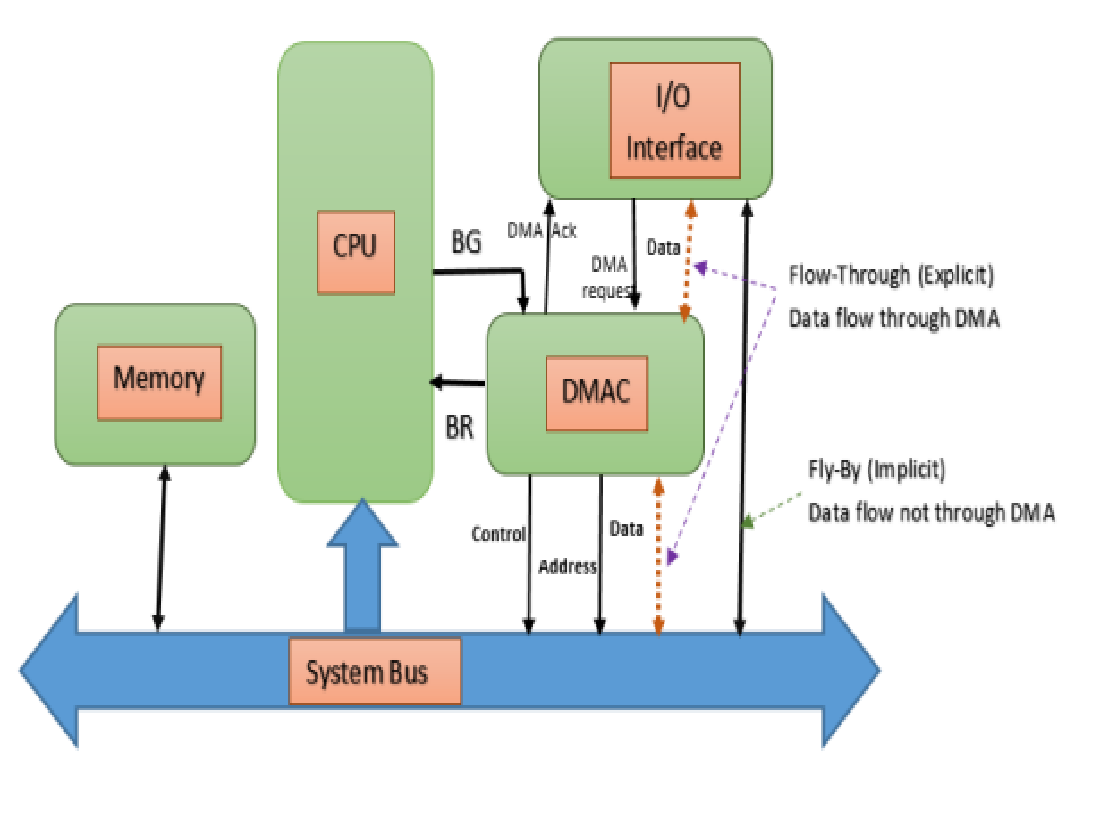
\includegraphics[width=0.70\textwidth]{graphics/DMA.png}
    \caption{Data transfer for a DMA controller. Where the data transfers from the I/O device directly to memory. \cite{ahmed_design_2019}}
    \label{fig:DMAcontroller}
\end{figure}

Bus request (BR) signal is sent to the processor during the data transfer operation.
The processor then finishes its current job and replies with a bus grant (BG) signal.
The DMA controller receives the signal and can then initiate the data transfer.
There are two modes in which the DMA can perform data transfers.
The first is called flow through, where the data flows through the DMA controller between the I/O device to memory.
The second is called fly by, where the data is transferred directly between the I/O device and memory \cite{ahmed_design_2019}.


%%% Local Variables: 
%%% mode: latex
%%% TeX-master: "DEGREE-NAME-YEAR"
%%% End: 
